\documentclass[manuscript,review]{acmart}

\usepackage{graphicx}
\usepackage{booktabs}
\usepackage{amsmath}
\let\Bbbk\relax   % kills the "\Bbbk already defined" clash with newtxmath (acmart)
\usepackage{amssymb}
\usepackage{xspace}
\usepackage{multirow}

\usepackage{algorithm}
\usepackage{algpseudocode}
\usepackage{tikz}
\usetikzlibrary{shapes.geometric, arrows.meta, positioning, calc, fit, backgrounds}

\graphicspath{{figures/}}

% drop the copyright block + acm reference format, not needed here
\settopmatter{printacmref=false}
\renewcommand\footnotetextcopyrightpermission[1]{}
\pagestyle{plain}
\setcopyright{none}
\acmConference[Reproduction Report]{CSE 200: Technical Writing and
Presentation}{January 2026 Term}{Dhaka, Bangladesh}
\acmYear{2026}
\copyrightyear{2026}

\newcommand{\nf}{NanoFlow\xspace}   % so I don't retype this everywhere
\newcommand{\Bdense}{B_{\mathrm{Dense}}}
\newcommand{\Pmodel}{P_{\mathrm{Model}}}
\newcommand{\Dmodel}{D_{\mathrm{model}}}
\newcommand{\membw}{\mathrm{MemBW}}
\newcommand{\memsize}{\mathrm{MemSize}}
\newcommand{\compute}{\mathrm{Compute}}
\newcommand{\netbw}{\mathrm{NetBW}}

\begin{document}

\title{NanoFlow: Towards Optimal Large Language Model Serving Throughput}

\author{Kan Zhu}
\affiliation{%
  \institution{University of Washington}
  \country{USA}
}

\author{Yufei Gao}
\affiliation{%
  \institution{University of Washington}
  \institution{Tsinghua University}
  \country{USA}
}

\author{Yilong Zhao}
\affiliation{%
  \institution{University of Washington}
  \institution{UC Berkeley}
  \country{USA}
}

\author{Liangyu Zhao}
\affiliation{%
  \institution{University of Washington}
  \country{USA}
}

\author{Gefei Zuo}
\affiliation{%
  \institution{University of Michigan}
  \country{USA}
}

\author{Yile Gu}
\affiliation{%
  \institution{University of Washington}
  \country{USA}
}

\author{Dedong Xie}
\affiliation{%
  \institution{University of Washington}
  \country{USA}
}

\author{Tian Tang}
\affiliation{%
  \institution{University of Washington}
  \institution{Tsinghua University}
  \country{USA}
}

\author{Qinyu Xu}
\affiliation{%
  \institution{University of Washington}
  \institution{Tsinghua University}
  \country{USA}
}

\author{Zihao Ye}
\affiliation{%
  \institution{University of Washington}
  \country{USA}
}

\author{Keisuke Kamahori}
\affiliation{%
  \institution{University of Washington}
  \country{USA}
}

\author{Chien-Yu Lin}
\affiliation{%
  \institution{University of Washington}
  \country{USA}
}

\author{Ziren Wang}
\affiliation{%
  \institution{University of Washington}
  \institution{Tsinghua University}
  \country{USA}
}

\author{Stephanie Wang}
\affiliation{%
  \institution{University of Washington}
  \country{USA}
}

\author{Arvind Krishnamurthy}
\affiliation{%
  \institution{University of Washington}
  \country{USA}
}

\author{Baris Kasikci}
\affiliation{%
  \institution{University of Washington}
  \country{USA}
}

\renewcommand{\shortauthors}{Zhu et al.}

\begin{abstract}
Large Language Models (LLMs) have resulted in a surging demand for planet-scale serving systems, 
where tens of thousands of GPUs continuously serve hundreds of millions of users. Consequently, 
throughput has emerged as a key metric that determines serving systems' performance. Due to large model 
sizes and memory-intensive self-attention, LLM serving has been commonly assumed to be memory-bound. 
Through a detailed analysis, we show that despite having memory-intensive components, end-to-end LLM 
serving is compute bound for most common workloads and LLMs. Alas, most existing serving engines fall short
from optimal compute utilization, because the heterogeneous operations that comprise LLM serving---compute,
memory, networking---are executed sequentially within a device.

We propose NanoFlow, a novel serving framework that exploits intra-device parallelism, which overlaps the 
usage of heterogeneous resources within a single device. NanoFlow splits inputs into smaller nano-batches 
and duplicates operations to operate on each portion independently, enabling overlapping. NanoFlow 
automatically identifies the number, size, ordering, and GPU resource allocation of nano-batches to 
minimize the execution time, while considering the interference of concurrent operations. We evaluate 
NanoFlow's end-to-end serving throughput on several popular models such as LLaMA-2-70B, Mixtral 
8$\times$7B, LLaMA-3-8B, etc. With practical workloads, NanoFlow provides 1.91$\times$ throughput boost 
compared to state-of-the-art serving systems, achieving between 50\% to 72\% of optimal throughput across 
popular models.
\end{abstract}

\keywords{Large Language Models, Inference Serving, Throughput, GPU Utilization, Intra-device Parallelism, 
Nano-batching, Pipeline Scheduling}

\maketitle

\section{Introduction}

Transformer-based large language models now sit behind chatbots, search, and office 
autocomplete~\cite{mehdi2023bing, openai2023chatgpt, spataro2023copilot}, with weekly ChatGPT usage 
reportedly in the hundreds of millions~\cite{patel2023inference, roth2024chatgpt, singh2024statistics}. 
Every interaction consumes scarce, expensive GPU time~\cite{griffith2023hunt, tingfang2023tsmc}, so 
operators optimize for a single objective---tokens per second per device. Throughput has become the 
dominant cost metric~\cite{kwon2023efficient, holmes2024deepspeed, nvidia2024tensorrt}.

Serving an LLM is structurally harder than serving earlier networks. Model weights are 
enormous---GPT-3's 175B parameters need roughly five 80\,GB A100s just for FP16 
weights~\cite{brown2020language}---and self-attention~\cite{vaswani2017attention} adds per-request state 
that grows with context length. Production systems cache per-request keys and values in a 
\emph{KV-cache}~\cite{pope2023efficiently} to avoid recomputation, but for long-context workloads that 
cache can exceed the weights themselves~\cite{tang2024quest}. Because a decode step reads all weights plus 
the entire KV-cache to emit one token per sequence, its arithmetic intensity looks terrible in isolation.

The field's natural conclusion is that serving is memory-bandwidth bound. The paper we reproduce argues this 
is wrong at the granularity that matters, because it ignores \emph{batching}. Once hundreds of requests are 
batched, weight-loading cost amortizes across the batch and the dense matrix multiplications that dominate a 
layer become arithmetic-limited rather than bandwidth-limited. Grouped-query attention~\cite{ainslie2023gqa} 
further shrinks per-request KV state so batches grow larger still, and as parameter counts climb the GEMM work 
grows faster than attention work. Evaluated end-to-end rather than operation-by-operation, mainstream serving 
sits firmly in a \emph{compute-bound} regime.

The corollary is uncomfortable: if compute binds, the right efficiency metric is achieved FLOP/s against 
hardware peak, and today's engines score poorly. Each kernel individually runs near 80\% of \emph{its own} 
bottleneck resource---a GEMM saturates tensor cores, decode attention saturates memory, an AllReduce saturates 
NVLink---but because they are dispatched sequentially onto one GPU, whichever resource limits throughput sits 
idle whenever another kernel runs. Aggregate compute utilization across a layer collapses to roughly 40\%.

\nf attacks this waste with intra-device parallelism: it runs operations of \emph{different} resource classes 
concurrently on one device, so a compute-bound GEMM and a memory-bound attention kernel occupy disjoint hardware 
at the same instant. To break the data dependency that serializes them, \nf splits each batch into 
\emph{nano-batches} and replicates each operation into \emph{nano-operations}, one per nano-batch. Because 
nano-batches hold disjoint requests, their nano-operations are independent and freely interleavable. Splitting 
into $k$ nano-batches reloads weights $k$ times, raising memory traffic; the arbitrage is that a compute-bound 
workload has idle memory bandwidth, so the extra loads hide in memory-idle windows at no wall-clock cost. \nf 
further hands each nano-operation only a \emph{fraction} of the GPU's SMs, since bandwidth-bound kernels 
saturate with far fewer thread blocks than compute-bound ones.

Building this raises two problems. \emph{The scheduling search space is enormous}: the number, size, and 
ordering of nano-operations depend on hidden dimension, layer count, GQA/MoE structure, the GPU's 
compute-to-bandwidth ratio, and the prefill/decode mix---hand-tuning per (model, hardware, workload) does 
not scale. \emph{Concurrent kernels interfere unpredictably}: two kernels sharing an SM contend for warp 
slots, L2, and memory-controller queues~\cite{strati2024orion}, and the slowdown is non-linear and asymmetric. 
NVIDIA GPUs expose no interface to partition compute, bandwidth, and network directly, so the trade-off must 
be inferred empirically.

\nf resolves both with \emph{auto-search}, a two-stage MILP optimizer. Stage~I ignores interference and solves 
the pipeline structure---counts, sizes, and ordering of nano-operations---keeping the combinatorial part 
tractable. Stage~II fixes that structure and allocates each concurrent nano-operation a GPU fraction using an 
empirically profiled interference model. A runtime forms batches asynchronously, enforces the ordering with CUDA 
events, and offloads KV-cache to a CPU/SSD hierarchy. On LLaMA-2-70B across eight A100s, \nf reaches 68.5\% of 
the cost-model optimum, averages a 1.91$\times$ throughput gain over TensorRT-LLM on realistic traces 
(ShareGPT, LMSYS-Chat-1M, Splitwise), and sustains 1.64$\times$ the request rate of the best baseline within a 
200\,ms latency SLO. Auto-search generalizes without manual tuning to LLaMA-3-8B/70B, Qwen2-72B, Deepseek-67B, 
and Mixtral 8$\times$7B, reaching 50--72\% of optimal on each.

The original work's contributions, restated:

\begin{itemize}
  \item An analytical cost model of LLM serving---validated against kernel
        measurements---that establishes modern workloads as compute-bound and
        yields a closed-form optimal-throughput expression.
  \item \nf: an MILP auto-search engine that discovers intra-device pipelines
        automatically, plus an end-to-end runtime that executes them.
  \item An evaluation showing 1.91$\times$ throughput over state-of-the-art
        baselines, at 68.5\% of the derived ceiling, across six architectures.
\end{itemize}

\noindent Section~\ref{sec:background} covers the inference workflow and
operation classification; Section~\ref{sec:method} presents the cost model and
\nf's design; Section~\ref{sec:results} reports results; and
Section~\ref{sec:discussion} offers a critical assessment.

\section{Background and Related Work}
\label{sec:background}

\subsection{The LLM Inference Workflow}

Contemporary production models---GPT-4, LLaMA, Mistral~\cite{openai2024gpt4, meta2024llama3, 
touvron2023llama2}---are decoder-only transformers~\cite{vaswani2017attention} served in two 
phases~\cite{yu2022orca}. \emph{Prefill} ingests the whole prompt at once as a single large matrix, writing 
keys and values into the KV-cache. \emph{Decode} then generates one token at a time, each step conditioned on 
all prior tokens, with the KV-cache sparing decode step $t$ from recomputing keys and values for 
tokens $1 \ldots t{-}1$~\cite{pope2023efficiently}.

Both phases traverse the same stack of identical decoder layers (Figure~\ref{fig:transformer}). Within a layer, 
the input activation is projected by $W_Q$, $W_K$, $W_V$ into queries, keys, and values; the new keys/values are 
appended to the KV-cache. The query is scored against every cached key, normalized into attention weights, and 
used to form a convex combination of cached values, which passes through the output projection $W_O$ and a layer 
norm~\cite{ba2016layernorm}. The feed-forward block then projects the activation through $W_{up}$ and $W_{gate}$,
 applies a nonlinearity such as SiLU~\cite{elfwing2017sigmoid} to the gate and multiplies elementwise, and 
 projects back through $W_{down}$ to the model dimension for the next layer.

\begin{figure}[t]
  \centering
  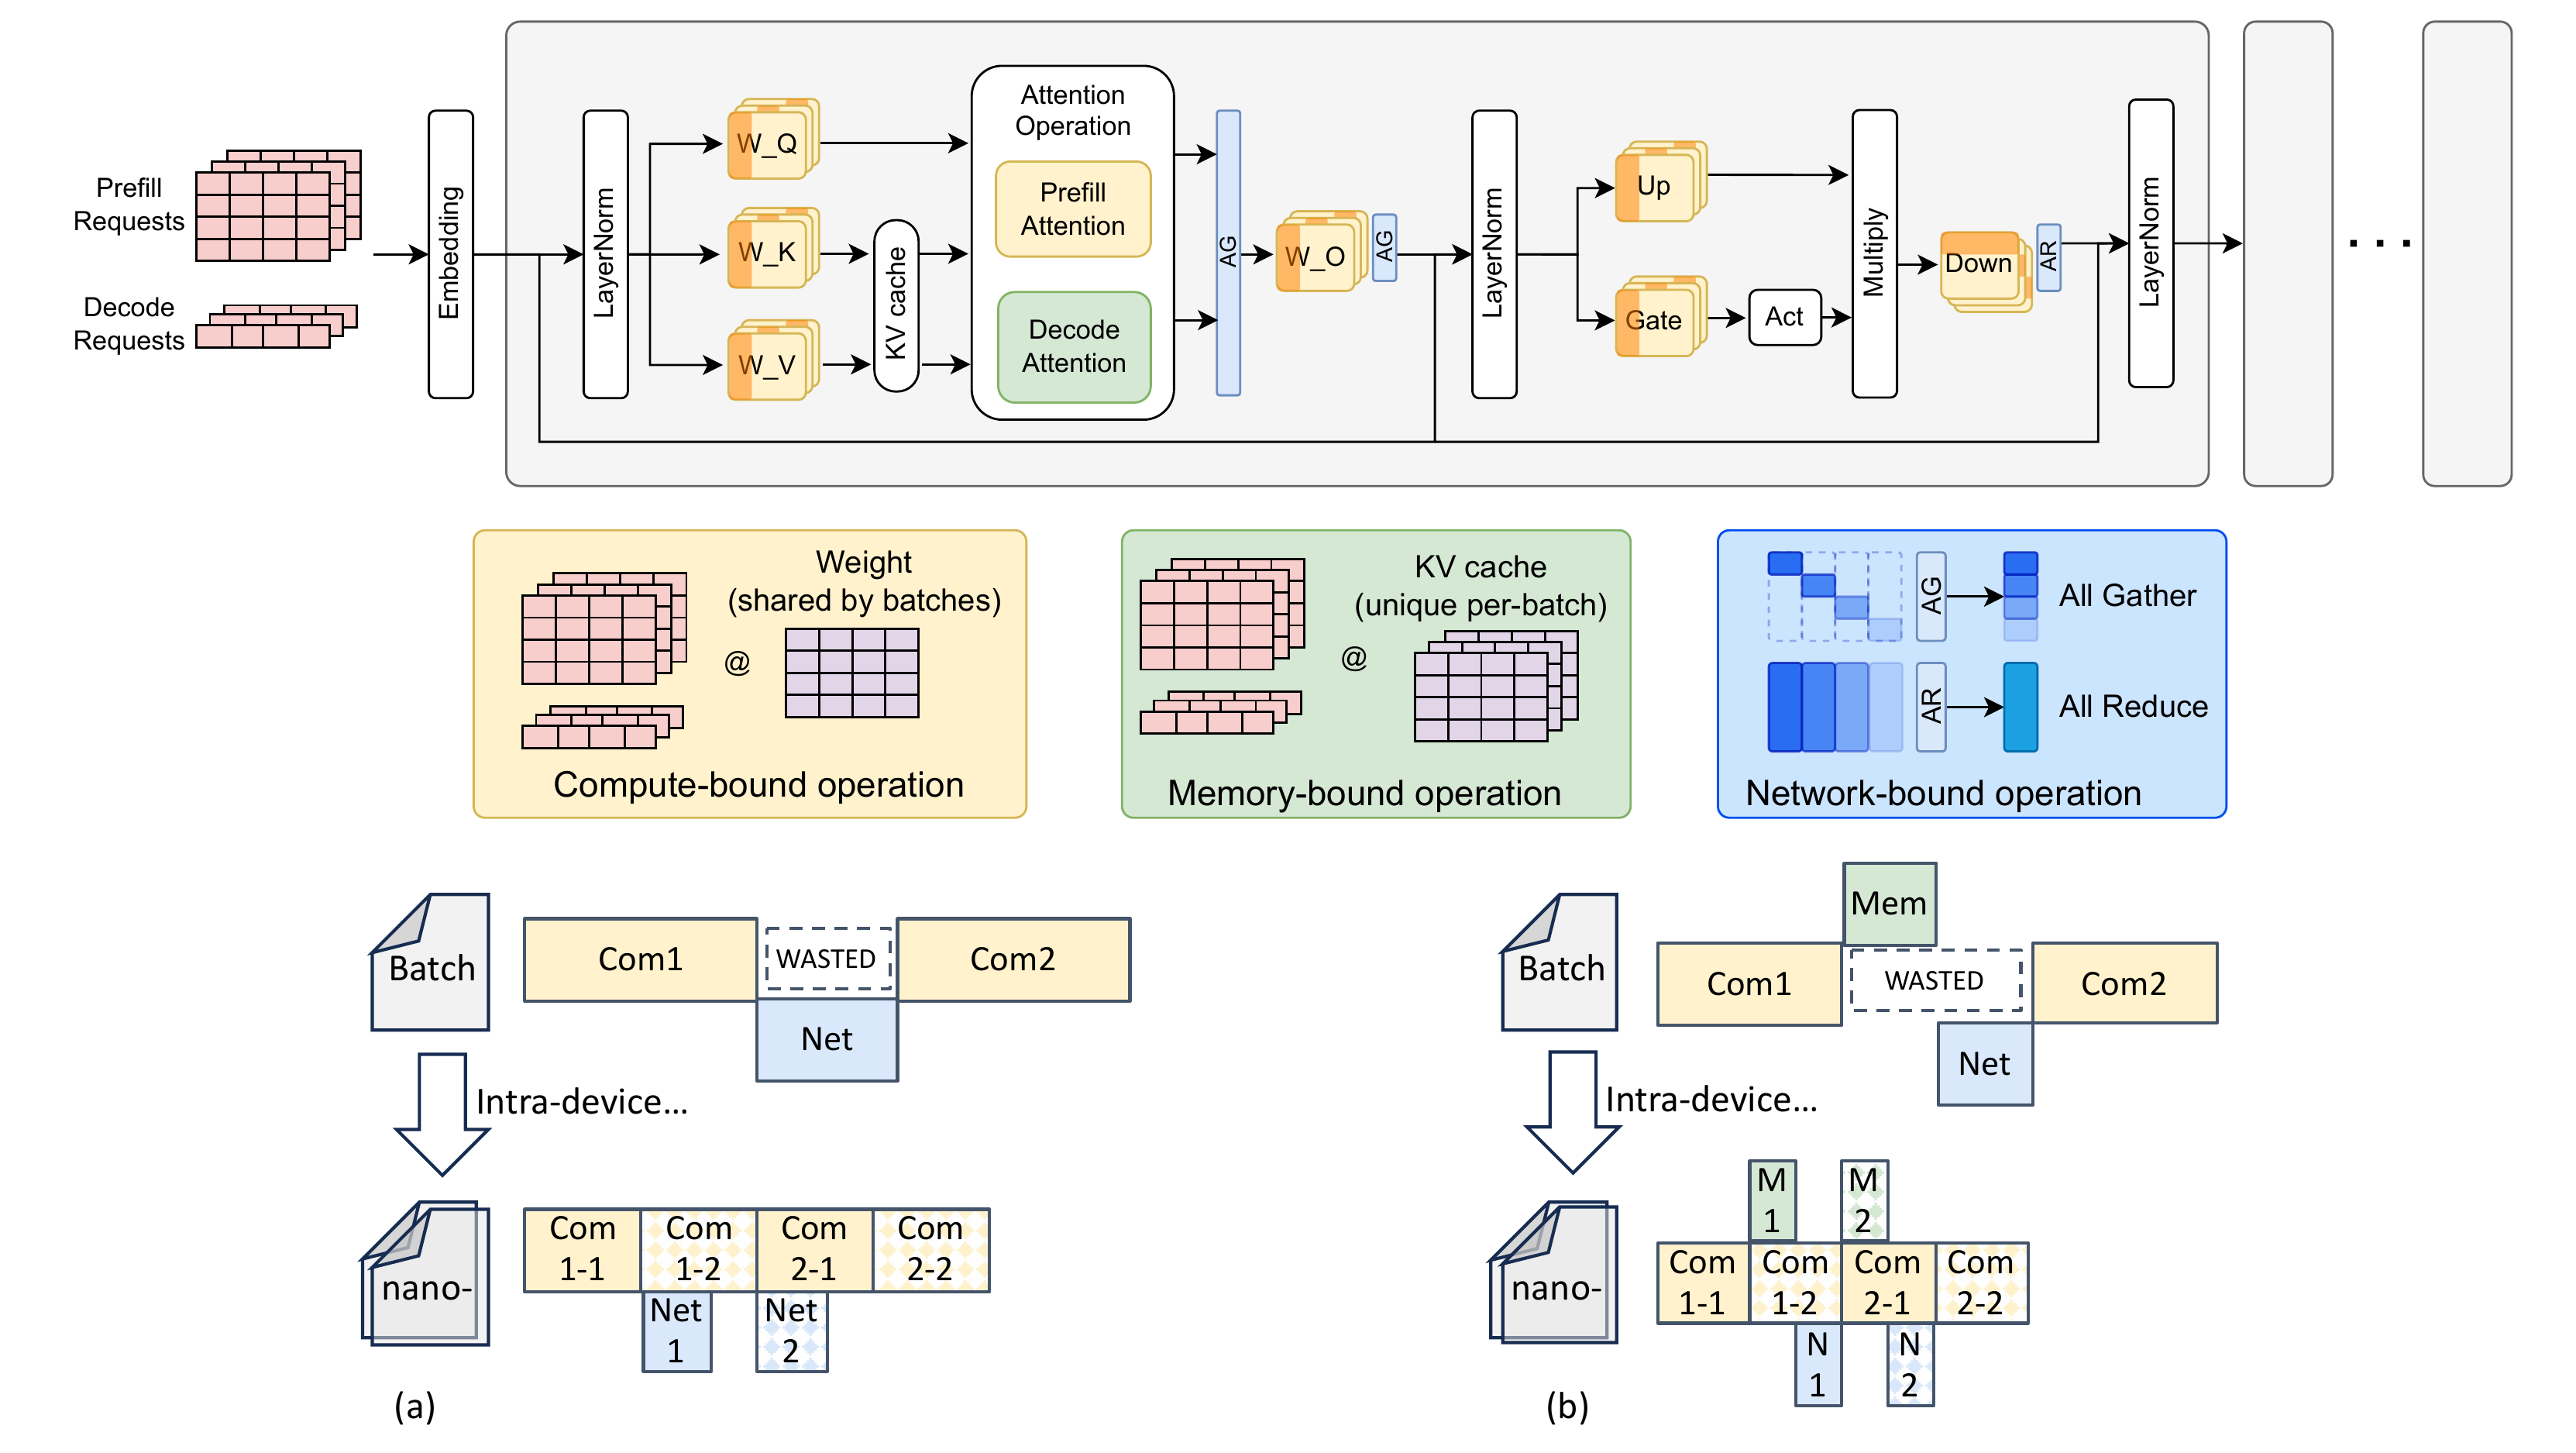
\includegraphics[width=\linewidth]{fig1_transformer.png}
  \caption{Transformer architecture, reproduced from the original paper. The operations in the yellow boxes 
  have large batch sizes and share model weight parameters across requests; hence, they are compute-bound. 
  Operations in green boxes require loading a unique KV cache for each request; hence, they are memory-bound. 
  The blue box represents network operations that perform synchronization between operations.}
  \label{fig:transformer}
\end{figure}

\subsection{Classifying Operations by Bottleneck Resource}
\label{sec:opchar}

The paper's central move is to sort a layer's operations by \emph{which hardware resource each saturates}. 
Four classes emerge.

\textbf{Dense operations.} KQV generation, the O-projection, and the Up/Gate/Down projections multiply 
activations against weight matrices. Prefill and decode use the same weights, so they fuse into one 
GEMM---chunked prefill~\cite{agrawal2023sarathi}---amortizing weight loading across a large batch. Dense 
operations are unambiguously \emph{compute-bound}.

\textbf{Attention operations.} Prefill attention scores a whole prompt against itself---a matrix-matrix product, 
\emph{compute-bound}. Decode attention scores a single query against a request-unique KV-cache---a matrix-vector 
product that reads a large tensor for few FLOPs, \emph{memory-bound}.

\textbf{Network operations.} Under tensor parallelism, per-layer partial results are reconciled across GPUs by 
AllGather (AG) and AllReduce (AR) collectives, limited by interconnect bandwidth 
(NVLink~\cite{nvidia2024nvlink}): \emph{network-bound}.

\textbf{Other operations.} Layer norms, positional embeddings, and activations---individually cheap, folded into 
a residual category.

The heterogeneity is the point: a GEMM and a decode-attention kernel stress disjoint hardware, so running them 
sequentially idles one resource while the other works. Running them concurrently---absent a data 
dependency---keeps both busy, which is exactly what \nf arranges.
\subsection{Multi-GPU Serving}

Large models do not fit on one device~\cite{li2023alpaserve}, so systems partition 
them~\cite{he2022fastermoe, shoeybi2020megatron, zheng2022alpa}. 
\textbf{Tensor parallelism}~\cite{shoeybi2020megatron, zheng2022alpa} 
shards each weight matrix across GPUs; every device participates in every operation, so compute and memory 
scale with device count, at the cost of a collective after nearly every operation 
(the AG/AR calls in Figure~\ref{fig:transformer}). \textbf{Pipeline parallelism}~\cite{huang2019gpipe} 
instead splits the model by depth, minimizing communication but introducing pipeline bubbles. In practice they 
compose---tensor parallelism within a node, pipeline across nodes---and this evaluation uses TP=8 within one 
DGX node.

\subsection{Related Work}
\label{sec:related}

\textbf{Serving optimizations at coarser granularities.} Prior work attacks serving efficiency 
above the individual operation. Orca~\cite{yu2022orca} introduced continuous batching at iteration 
granularity; DistServe~\cite{zhong2024distserve} and Splitwise~\cite{patel2023splitwise} disaggregate prefill 
and decode onto separate clusters; DeepSpeed-FastGen~\cite{holmes2024deepspeed} and 
Sarathi-Serve~\cite{agrawal2024sarathi} chunk prefills and co-batch them with decodes. All schedule 
\emph{requests}, none schedules \emph{operations}, so none can co-locate a GEMM and a decode-attention on the 
GPU---the gap \nf targets. A parallel thread improves individual kernels 
(PagedAttention~\cite{kwon2023efficient}, quantization~\cite{lin2024qserve, tang2024quest, zhao2023atom}); 
\nf is complementary, since a better kernel is simply re-profiled into auto-search.

\textbf{Operator-level parallelism in DNN compilers.} Rammer~\cite{ma2020rammer}, Unity~\cite{unger2022unity}, 
ASPEN~\cite{park2023aspen}, and Welder~\cite{shi2023welder} expose intra-operator parallelism or dissolve 
operator boundaries into tile-level dataflow, but optimize for parallelism without modeling that different 
operators are limited by \emph{different physical resources}; their tiles inherit the graph's sequential 
dependencies, capping expressible overlap, and they generally demand per-model recompilation. 
\nf's nano-batching sidesteps the dependency problem by construction, and auto-search removes the manual effort.

\section{Method}
\label{sec:method}

This section develops the cost model that identifies the bottleneck and validates it
(\S\ref{sec:costmodel}--\S\ref{sec:validation}), the optimal-throughput bound and the gap real systems 
leave (\S\ref{sec:optimal}--\S\ref{sec:gap}), then \nf's mechanism (\S\ref{sec:intradevice}), auto-search 
(\S\ref{sec:autosearch}), and runtime (\S\ref{sec:runtime}).

\subsection{A Cost Model for LLM Serving}
\label{sec:costmodel}

\subsubsection{Parameters}

Throughput means \emph{total} tokens per second, prefill and decode alike, governed by four parameter groups.

\textbf{Hardware.} $N_{\mathrm{GPU}}$; $\membw$ (aggregate bandwidth); $\memsize$ (capacity);
$\compute$ (aggregate FLOP/s); $\netbw$ (interconnect bandwidth).

\textbf{Model.} $\Dmodel$ (hidden dimension); $L$ (layers); $\Pmodel$ (parameters);
$R_{\mathrm{GQA}}$; $S_{\mathrm{type}}$ (bytes/parameter, 2 for FP16).

\textbf{Workload.} $p$ (mean prompt tokens), $d$ (mean generated tokens); a request
contributes $p+d$ tokens, so decode throughput is
$d/(p+d)\,\mathrm{Throughput}_{\mathrm{total}}$ and request rate is
$1/(p+d)\,\mathrm{Throughput}_{\mathrm{total}}$.

\textbf{Batch size.} The model assumes the largest batch memory permits---weights plus every active request's 
KV-cache---which is right for a throughput-oriented system: larger batches amortize weight loading and dilute 
fixed launch costs. Activations are neglected ($<$5\% of memory~\cite{kwon2023efficient}).

\subsubsection{Latency from Three Perspectives}

Under the max-batch assumption, one iteration (a full forward pass through all $L$ layers) can be costed three 
ways.

\textbf{Memory.} At max batch, essentially all device memory is touched once per iteration---weights streamed 
in, every KV-cache read by decode attention---and cross-iteration weight caching is hopeless because the reuse 
distance spans the whole forward pass:
\begin{equation}
  T_{\mathrm{mem}} = \frac{\memsize}{\membw}.
  \label{eq:tmem}
\end{equation}

\textbf{Compute.} Dense operations dominate FLOPs (validated in
\S\ref{sec:validation}). A GEMM against a weight matrix $N_w \times K_w$ at batch
$\Bdense$ costs $2\Bdense N_w K_w$ FLOPs; summing over all weight matrices gives
$2\Bdense \sum N_w K_w$, and $\sum N_w K_w = \Pmodel$. Therefore
\begin{equation}
  T_{\mathrm{compute}} \approx \frac{2 \Bdense \cdot \Pmodel}{\compute}.
  \label{eq:tcompute}
\end{equation}
Crucially, compute time depends on the parameter count and nothing else about the
architecture.

\textbf{Network.} Tensor parallelism moves, per layer, two AllGathers and one
AllReduce~\cite{shoeybi2020megatron_b} over $[\Bdense, \Dmodel]$ activations,
totaling $4\,\Bdense \Dmodel S_{\mathrm{type}}$ per-GPU bytes per layer:
\begin{equation}
  T_{\mathrm{net}} \approx 4 \cdot
    \frac{N_{\mathrm{GPU}}\, \Bdense\, \Dmodel\, S_{\mathrm{type}}\, L}{\netbw}.
  \label{eq:tnet}
\end{equation}

\subsection{Which Resource Actually Binds?}
\label{sec:classification}

\subsubsection{Network versus Compute}

Dividing Eq.~\ref{eq:tnet} by Eq.~\ref{eq:tcompute}:
\begin{equation}
  \frac{T_{\mathrm{net}}}{T_{\mathrm{compute}}}
    = \frac{2 \Dmodel L}{\Pmodel} \cdot
      \frac{N_{\mathrm{GPU}} \cdot \compute}{\netbw / S_{\mathrm{type}}}.
  \label{eq:netratio}
\end{equation}
Standard parameter accounting (with intermediate dimension
$3.5\times\Dmodel$~\cite{jiang2023mistral, meta2024llama3}) gives
$\Pmodel \approx 12\Dmodel^2 L$, collapsing the first factor to
$\approx 1/(6\Dmodel)$. Any model needing multiple GPUs has
$\Dmodel > 4096$~\cite{cloud2024qwen2, jiang2023mistral, meta2024llama3,
touvron2023llama}, so this factor is below $10^{-5}$, while modern interconnects
(NVLink~\cite{nvidia2024nvlink}, Infinity Fabric~\cite{zhao2024forestcoll}) put
the second factor at $10^4$--$10^5$. The product lands below 1:
\emph{the network is not the bottleneck}.

\subsubsection{Memory versus Compute}

The decisive comparison. Dividing Eq.~\ref{eq:tmem} by Eq.~\ref{eq:tcompute}:
\begin{equation}
  T_R = \frac{T_{\mathrm{mem}}}{T_{\mathrm{compute}}}
      \approx \frac{\compute}{\membw} \cdot
              \frac{\memsize}{\Pmodel} \cdot
              \frac{1}{2 \Bdense}.
  \label{eq:tr}
\end{equation}
$T_R < 1$ means compute-bound.

Two trends push $T_R$ down. \emph{GQA}~\cite{ainslie2023gqa}---now standard in 
LLaMA-3~\cite{touvron2023llama}, NeMo~\cite{mistral2024nemo}, and 
Qwen2~\cite{cloud2024qwen2}---shrinks per-request KV state so far more requests fit, raising 
$\Bdense$; the authors report LLaMA-2-70B on 8$\times$A100 sustaining $\Bdense \approx 2048$ 
where a non-GQA model would manage 256, an 8$\times$ swing. \emph{Model growth} only increases 
$\Pmodel$ in the denominator. Across five models and six workloads nearly every $T_R$ is below 1 
(compute-bound); the lone exception is LLaMA-3-8B under a long-decode (512-in/1024-out) workload, 
where $T_R \approx 1$. Table~\ref{tab:accelerators} reproduces the accelerator survey: the ratios 
that matter ($\compute/\membw$, $\netbw/\membw$) are remarkably stable across vendors and eight years of silicon, 
so the conclusion is not A100-specific.

\begin{table*}[t]
\centering
\caption{Characteristics of accelerator models across various vendors and release years. Recreated from 
Table~1 of the original paper. The three rightmost columns are the ratios that matter: they are conspicuously 
flat across a decade of hardware, which is why the compute-bound conclusion is not A100-specific.}
\label{tab:accelerators}
\small
\begin{tabular}{llrrrrrrrr}
\toprule
\textbf{Vendor} & \textbf{Model} & \textbf{Release} & \textbf{MemSize} &
\textbf{MemBW} & \textbf{NetBW} & \textbf{Compute} &
$\dfrac{\memsize}{\membw}$ & $\dfrac{\compute}{\membw}$ &
$\dfrac{\netbw}{\membw}$ \\
 & & \textbf{Year} & \textbf{(GB)} & \textbf{(GB/s)} & \textbf{(GB/s)} &
\textbf{(FP16 GFLOP/s)} & & & \\
\midrule
NVIDIA & V100        & 2017 & 16  & 900   & 300   & 125{,}000   & 0.018 & 139 & 0.33  \\
NVIDIA & A100 (40GB) & 2020 & 40  & 1{,}555 & 600 & 312{,}000   & 0.026 & 200 & 0.39  \\
NVIDIA & A100 (80GB) & 2021 & 80  & 2{,}000 & 600 & 312{,}000   & 0.040 & 156 & 0.30  \\
NVIDIA & H100        & 2023 & 80  & 3{,}352 & 900 & 989{,}000   & 0.024 & 295 & 0.268 \\
NVIDIA & H200        & 2024 & 96  & 4{,}800 & 900 & 989{,}000   & 0.020 & 206 & 0.19  \\
NVIDIA & B100        & 2024 & 120 & 8{,}000 & 1{,}800 & 1{,}800{,}000 & 0.015 & 225 & 0.23 \\
NVIDIA & B200        & 2024 & 120 & 8{,}000 & 1{,}800 & 2{,}250{,}000 & 0.015 & 281 & 0.23 \\
AMD    & MI250       & 2021 & 128 & 3{,}352 & 800 & 362{,}000   & 0.038 & 107 & 0.24  \\
AMD    & MI300       & 2023 & 192 & 5{,}300 & 1{,}024 & 1{,}307{,}000 & 0.036 & 246 & 0.19 \\
AMD    & MI325X      & 2024 & 256 & 6{,}000 & 1{,}024 & 1{,}307{,}000 & 0.043 & 218 & 0.17 \\
Intel  & Gaudi 2     & 2022 & 96  & 2{,}400 & 600 & 1{,}000{,}000 & 0.040 & 417 & 0.25 \\
Intel  & Gaudi 3     & 2024 & 128 & 3{,}700 & 1{,}200 & 1{,}800{,}000 & 0.035 & 486 & 0.32 \\
NVIDIA & Ada 6000    & 2022 & 48  & 960   & 64    & 182{,}000   & 0.050 & 190 & 0.067 \\
\bottomrule
\end{tabular}
\end{table*}

\subsection{Validating the Model}
\label{sec:validation}

The authors validate the model on LLaMA-2-70B, 8$\times$A100, $\Bdense = 2048$: per-operation FLOPs, bytes, 
and network traffic are fed through Eqs.~\ref{eq:tmem}--\ref{eq:tnet} and compared to measured kernel times 
(Table~\ref{tab:validation}). Predictions track measurement well; the one clear miss is prefill attention 
(0.37\,ms predicted vs.\ 4.56\,ms measured), which the authors attribute to kernel-launch overhead on a 
too-small kernel---an honest disclosure that does not move the aggregate. Summing the columns, 
$T_{\mathrm{compute}} = 114.17$\,ms exceeds $T_{\mathrm{mem}} = 45.09$\,ms by $2.5\times$ and $T_{\mathrm{net}} = 31.33$\,ms by 
$3.6\times$. Notably, 462\,GB of the memory load is decode attention alone---the very operation cited to call 
serving memory-bound. The operation is memory-bound; the layer is not.
\begin{table}[t]
\centering
\caption{Comparison of operation runtimes between cost model estimation and real-world measurements. 
Recreated from Table~2 of the original paper. LLaMA-2-70B, 8$\times$A100, $\Bdense = 2048$. UG = Up+Gate; 
D = Down; DecAttn = decode attention; PfAttn = prefill attention; $T_{\mathrm{comp}}$/$T_{\mathrm{mem}}$/$T_{\mathrm{net}}$ = estimated compute/memory/network time.}
\label{tab:validation}
\small
\setlength{\tabcolsep}{4pt}
\begin{tabular}{lrrrrrrr}
\toprule
\textbf{Op} & \textbf{Compute} & \textbf{Mem} & \textbf{Net} &
\textbf{Est.} & \textbf{Est.} & \textbf{Est.} & \textbf{Real} \\
 & \textbf{(GFLOP)} & \textbf{Load} & \textbf{Usage} &
$T_{\mathrm{comp}}$ & $T_{\mathrm{mem}}$ & $T_{\mathrm{net}}$ & \textbf{Time} \\
 & & \textbf{(GB)} & \textbf{(GB)} & \textbf{(ms)} & \textbf{(ms)} &
\textbf{(ms)} & \textbf{(ms)} \\
\midrule
KQV     & 27{,}487.8  & 19.5  & 0    & 11.01 & 1.22  & 0     & 16.08 \\
O       & 21{,}990.2  & 16.1  & 0    & 8.81  & 1.01  & 0     & 16.01 \\
UG      & 153{,}931.6 & 96.6  & 0    & 61.67 & 6.04  & 0     & 69.92 \\
D       & 76{,}965.8  & 49.7  & 0    & 30.84 & 3.11  & 0     & 34.96 \\
DecAttn & 3{,}665.9   & 462.2 & 0    & 1.47  & 28.89 & 0     & 35.60 \\
PfAttn  & 916.3       & 2.1   & 0    & 0.37  & 0.13  & 0     & 4.56  \\
Net     & 18.8        & 75.2  & 75.2 & 0.01  & 4.70  & 31.33 & 47.92 \\
\midrule
\textbf{Total} & & & & \textbf{114.17} & \textbf{45.09} & \textbf{31.33} & \\
\bottomrule
\end{tabular}
\end{table}

\subsection{The Optimal Throughput Bound}
\label{sec:optimal}

If compute is the binding constraint, peak throughput is achieved exactly when
the tensor cores never idle. Rearranging Eq.~\ref{eq:tcompute}:
\begin{equation}
  \mathrm{Throughput}_{\mathrm{optimal}}
    = \frac{\Bdense}{T_{\mathrm{compute}}}
    = \frac{\compute}{2 \Pmodel}.
  \label{eq:optimal}
\end{equation}

Two quantities set the ceiling---aggregate FLOP/s and parameter count. Memory capacity, bandwidth, 
prompt length, and generation length all drop out; they determine only how close an implementation gets, 
not where the ceiling lies. For LLaMA-2-70B on 8$\times$A100, profiling CUTLASS~\cite{thakkar2023cutlass} 
gives a realistic 280\,TFLOPS FP16 peak, so with $\Pmodel = 70$B the ceiling is 1857 tokens/s/GPU---the 
line every evaluation bar is measured against.

\subsection{Where Existing Systems Lose}
\label{sec:gap}

Against 1857 tokens/s/GPU the incumbents deliver only vLLM 22.0\%, DeepSpeed-FastGen 22.9\%, and 
TensorRT-LLM 37.8\%---the best throws away nearly two-thirds of the machine. Figure~\ref{fig:existing_pipeline} 
shows why: systems like SGLang~\cite{zheng2024sglang}, vLLM~\cite{kwon2023efficient}, and 
DeepSpeed-FastGen~\cite{holmes2024deepspeed} run one batch through the layer executing operations 
\emph{in sequence}, each a barrier for the next. During the memory-bound decode attention and the network 
AllReduce, the tensor cores sit idle---the ``WASTED'' bubbles in the figure---and aggregate compute utilization 
lands near 40\%.

\begin{figure}[t]
  \centering
  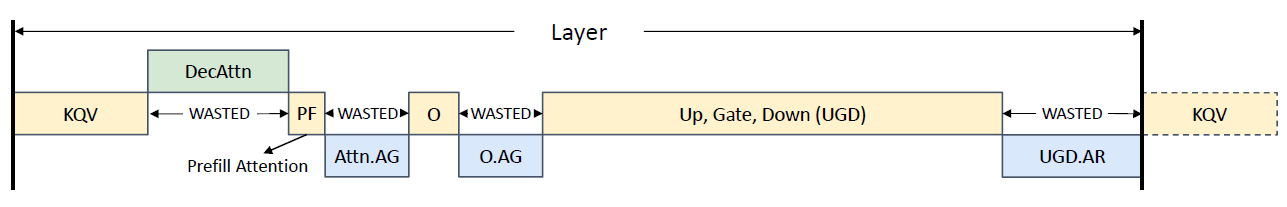
\includegraphics[width=\linewidth]{fig2_existing_pipeline.png}
  \caption{Execution pipeline of existing systems, reproduced from the original paper. Green, yellow, and 
  blue denote memory-, compute-, and network-bound operations respectively. ``WASTED'' marks the stages where 
  compute---the constrained resource---is underutilized.}
  \label{fig:existing_pipeline}
\end{figure}

\subsection{Intra-device Parallelism via Nano-batching}
\label{sec:intradevice}

The sequential design loads each weight matrix once; splitting the batch reloads them, which seems to add 
expensive memory traffic. But not in a compute-bound regime: \S\ref{sec:validation} showed memory bandwidth 
underutilized by more than half, so extra weight loads are charged against slack and, if overlapped with 
compute, cost zero wall-clock time. The system buys compute utilization with memory bandwidth it was not 
spending anyway.

\nf splits the batch: every operation becomes several nano-operations, bit-identical copies applied to 
disjoint \emph{nano-batches}. An Up projection over 2048 tokens becomes UP1 (tokens 0--767) and UP2 (768--2047). 
Because the nano-batches share no data, UP2 depends neither on UP1 nor on the decode attention of 
nano-batch~1---the serializing barrier is gone, and a compute-bound and a memory-bound nano-operation from 
different nano-batches can run concurrently on disjoint hardware.

Two details matter. First, \nf gives each nano-operation only a fraction $R$ of the SMs: bandwidth-bound 
kernels saturate at few thread blocks while GEMMs absorb every SM, so an 80/20 split costs the GEMM almost 
nothing. Second, KV-cache offload (\S\ref{sec:kvcache}) is scheduled into compute-bound windows where PCIe 
traffic is invisible.

Algorithm~\ref{alg:nanoflow} states the end-to-end procedure.

\begin{algorithm}[t]
\caption{\nf: Auto-search and Runtime Execution}
\label{alg:nanoflow}
\begin{algorithmic}[1]
\Require Model architecture $\mathcal{M}$, hardware spec $\mathcal{H}$,
         workload statistics $\mathcal{W} = (p, d)$
\Ensure  Optimized intra-device pipeline $\Pi$, served token stream

\Statex \textbf{Phase 0: Profiling (offline, once per model+hardware)}
\State $\Bdense \gets \Call{MaxDenseBatch}{\mathcal{M}, \mathcal{H}, \mathcal{W}}$
       \Comment{largest batch fitting in memory}
\ForAll{$k \in \{\text{GEMM}, \text{GEMV}, \text{Network}\}$}
  \ForAll{$b \in \{128, 256, \ldots, \Bdense\}$}
    \State $D_{\mathrm{best}}[k, b] \gets \min_{\text{impl}}
            \Call{ProfileIsolated}{k, b, \text{impl}}$
  \EndFor
\EndFor
\State $\mathcal{T}_{R \to P} \gets \Call{ProfilePairwiseInterference}{ }$
       \Comment{build Table~\ref{tab:interference}}

\Statex \textbf{Phase 1: Pipeline structure search (MILP, no interference)}
\State $n \gets 2$ \Comment{start with 2 nano-ops per operation}
\State $\Pi \gets \emptyset$
\Repeat
  \State $\Pi' \gets \Call{SolveMILP}{n, \Bdense, \mathcal{G}_{\mathrm{dep}}, D_{\mathrm{best}}}$
  \Statex \hspace{\algorithmicindent}
          \textbf{minimize} makespan \textit{s.t.}
          dependency, batch-size, and
  \Statex \hspace{\algorithmicindent}
          disjoint-resource-overlap constraints
  \If{$\Call{Makespan}{\Pi'} < \Call{Makespan}{\Pi}$}
    \State $\Pi \gets \Pi'$
  \EndIf
  \State $n \gets n + 1$ \Comment{split further near remaining bubbles}
\Until{no improvement in $\Call{Makespan}{\Pi}$}

\Statex \textbf{Phase 2: Resource allocation refinement (MILP, with interference)}
\State Fix counts, sizes, and ordering from $\Pi$
\State $\{R_i\} \gets \Call{SolveMILP}{\Pi, \mathcal{T}_{R \to P}}$
\Statex \hspace{\algorithmicindent}
        \textbf{minimize} makespan \textit{s.t.}
        $\sum_{i \in \text{concurrent}(t)} R_i \le 1.0\ \forall t$,
\Statex \hspace{\algorithmicindent}
        exec time of nano-op $i$ $= D_{\mathrm{best}}[i] / P(R_i)$
\State $\Pi \gets \Call{Annotate}{\Pi, \{R_i\}}$

\Statex \textbf{Phase 3: Runtime serving (online)}
\While{requests arrive}
  \State \textbf{asynchronously} form batch for iteration $i{+}1$
         \textit{while} GPU runs iteration $i$
  \State Prioritize unfinished decodes; chunk prefills to fill $\Bdense$ exactly
  \State Predict peak memory; admit new prefills only if within budget
  \ForAll{layer $\ell = 1 \ldots L$}
    \ForAll{nano-op $o \in \Pi$ \textbf{in order}}
      \State Launch kernel impl. for $(o, R_o)$; enforce deps via CUDA events
      \State Offload KV of $\ell$ to CPU/SSD during FFN compute window
    \EndFor
  \EndFor
  \State Detect EOS from iteration $i{-}1$; retire finished requests
\EndWhile
\State \Return served token stream
\end{algorithmic}
\end{algorithm}

\subsection{Auto-search}
\label{sec:autosearch}

\subsubsection{Profiling and the Interference Model}

Auto-search needs two inputs.

\textbf{Isolated kernel timings.} \nf profiles GEMM (dense), GEMV (decode attention), and network kernels at 
batch sizes $128 \ldots \Bdense$ in steps of 128, sweeping block/warp/tile configurations and recording the 
fastest implementation per (kernel, batch size).

\textbf{Interference.} Harder: GPUs offer no clean way to hand each nano-operation a fixed fraction of compute, 
bandwidth, and network. Co-running kernels contend for SMs, warp slots, L2, and memory-controller 
queues~\cite{strati2024orion}, and the slowdown is not predictable from first principles. \nf defines a 
\emph{proxy}: it measures how much a co-running kernel degrades GEMM performance and calls that GEMM's 
share $R$. If a co-scheduled GEMM runs at 40\% of isolated speed, $R_A = 0.4$ and the partner gets 
$R_B = 1 - R_A = 0.6$; the definition is GEMM-centric because compute is what \nf maximizes. Separately, 
$P$ is each kernel's achieved performance normalized to its isolated peak: $P_A = R_A$ for the GEMM by 
construction, while $P_B$ says how much memory/network throughput the partner achieves. The mapping 
$R \mapsto P$ is thus an \emph{exchange rate} between compute surrendered and memory/network gained.

Exhaustive profiling is infeasible, so \nf prunes hard: GEMV and network kernels are limited to 8--128 thread 
blocks (128 saturates their bandwidth); dominated GEMM implementations are discarded; and only \emph{pairwise} 
interference is profiled, assumed to hold under three-way overlap.

Table~\ref{tab:interference} distills the result, and its key feature is \emph{convexity}: surrendering the 
first 20\% of GEMM performance ($R = 1.0 \to 0.8$) buys 30\% of GEMV or 50\% of network performance, while the 
exchange rate turns unfavorable only at the far end. A scheduler that exploits only the cheap end of the curve 
captures most of the overlap benefit for little compute sacrifice---and Stage~II's MILP finds where to stop. 
The mapping is stable to within 5\% across GEMM shapes and 64 batch combinations, so one table suffices.

\begin{table}[t]
\centering
\caption{Performance $P$ of GEMV and network kernels at different resource
utilization levels $R$. Recreated from Table~3 of the original paper. Note the
convexity: the first 20\% of GEMM performance surrendered buys 30\% GEMV or 50\%
network performance.}
\label{tab:interference}
\begin{tabular}{lccccccc}
\toprule
\multirow{2}{*}{\textbf{Operation}} &
\multicolumn{7}{c}{\textbf{Resource Utilization} ($R$)} \\
\cmidrule(lr){2-8}
 & \textbf{0} & \textbf{0.1} & \textbf{0.2} & $\cdots$ &
   \textbf{0.8} & \textbf{0.9} & \textbf{1} \\
\midrule
GEMM (by defn.) & 0 & 0.1 & 0.2 & $\cdots$ & 0.80 & 0.90 & 1 \\
GEMV            & 0 & 0.2 & 0.3 & $\cdots$ & 0.85 & 0.95 & 1 \\
Network         & 0 & 0.3 & 0.5 & $\cdots$ & 0.90 & 1.00 & 1 \\
\bottomrule
\end{tabular}
\end{table}

\subsubsection{Stage I: Pipeline Structure}

Stage~I solves the pipeline \emph{shape}---counts, sizes, ordering---via MILP over interference-free timings; 
interference is excluded to keep the problem tractable and corrected in Stage~II. The formulation:

\textbf{Objective.} Minimize makespan---eliminate the compute bubbles of
Figure~\ref{fig:existing_pipeline}.

\textbf{Nano-operation count.} At least 2 per operation (one cannot overlap with itself), but splitting erodes 
batching, so auto-search starts at 2, solves, and selectively increases the split only for operations adjacent 
to a remaining bubble, stopping when it stops helping.

\textbf{Batch sizes and timings.} Sizes from $\{128, \ldots, \Bdense\}$; timings from the isolated profile.

\textbf{Dependencies.} Two nano-operations are dependent iff their parents are dependent \emph{and} their token 
ranges intersect---so O-projection over tokens 0--255 depends on attention over 0--255 but not 256--511. This 
conjunctive rule generates the parallelism.

\textbf{Overlap.} Only operations of \emph{different} resource classes may overlap; two GEMMs sharing tensor cores 
gain nothing.

\textbf{Operation transformations.} Algebraically equivalent collectives (an AG can become an AR under a different 
sharding~\cite{shoeybi2020megatron_b, zheng2022alpa}) are enumerated, hence the ``AG to AR Transform'' in 
Figure~\ref{fig:nanoflow_pipeline}.
Rather than prove optimality, \nf accepts the first good feasible solution
($\approx$10 minutes).

\subsubsection{Stage II: Resource Allocation}

Stage~II freezes Stage~I's structure and solves a second MILP for the resource shares $\{R_i\}$, using 
Table~\ref{tab:interference} to map each $R_i$ to an achieved $P_i$ (and a concrete kernel implementation). 
Constraints: $\sum_i R_i \le 1.0$ at any instant; nano-operation $i$ takes $D_{\mathrm{best}}[i]/P(R_i)$; objective, 
minimize makespan. Auto-search reruns only when the architecture or workload statistics change 
materially---negligible against week-long deployments.

\subsubsection{Discovered Pipelines}

\textbf{70B-class models} (LLaMA-2/3-70B, Qwen2.5-72B, Deepseek-67B) differ in vocabulary, layer count, and 
KQV bias, but none perturbs the resource profile enough to change the schedule; auto-search converges to 
near-identical pipelines for all four. Figure~\ref{fig:nanoflow_pipeline} shows the LLaMA-2-70B result: at 
the layer head all three resource classes have work (KQV compute, decode-attention memory, the previous 
layer's AllReduce), so KQV is split \emph{four} ways; decode attention takes $R = 0.4$ and achieves 80\% of 
its peak---the convex bargain of Table~\ref{tab:interference}---while the compute-dominated FFN prioritizes 
GEMMs ($R = 0.9$) with two nano-operations.

\textbf{8B models} (LLaMA-3-8B) fit on one GPU---no network operations---so everything splits in two, 
overlapping decode attention against Up-Gate-Down. \textbf{MoE models} (Mixtral 8$\times$7B) have imbalanced 
expert load~\cite{jiang2023mistral}, so \nf uses tensor parallelism with a grouped-GEMM FFN and a gate-routing 
step; auto-search handles the modified graph without special-casing.

\begin{figure*}[t]
  \centering
  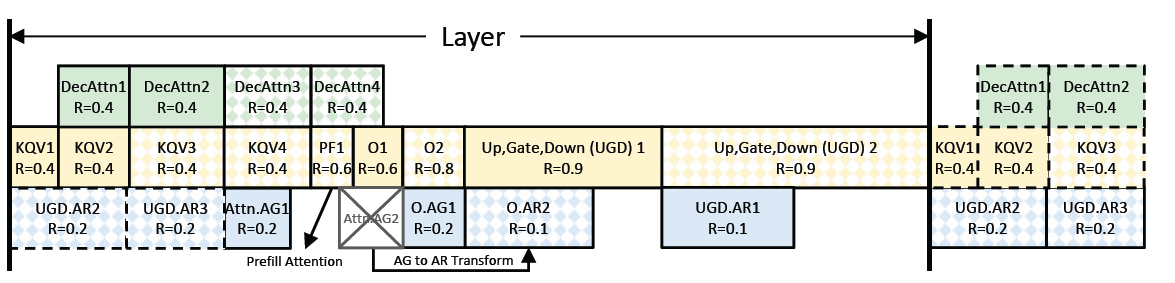
\includegraphics[width=\textwidth]{fig3_nanoflow_pipeline.png}
  \caption{Execution pipeline of LLaMA-2-70B, automatically generated by \nf; reproduced from the original paper.
  Solid and shaded backgrounds represent input batches 0--768 and 768--2048 respectively. $R$ denotes resource 
  utilization. Note the four-way KQV split at the head of the layer, where all three resource classes have work 
  available at once.}
  \label{fig:nanoflow_pipeline}
\end{figure*}

\subsection{The Runtime}
\label{sec:runtime}

\subsubsection{Request Scheduling}

\textbf{Batch formation.} \nf assumes autoscaling and routing are handled by an external control 
plane~\cite{jain2025router, patke2025chiron, aibrix2025} and that requests are plentiful. Following 
Sarathi-Serve~\cite{agrawal2023sarathi}, it prioritizes unfinished decodes, then chunks prefills at token 
granularity to hit a fixed best-performing $\Bdense$ every iteration. Constant batch shape stabilizes GEMM 
performance (p99 latency within 1.07$\times$ of mean) and self-balances---as decodes accumulate the prefill 
budget shrinks, and vice versa. To avoid OOM, \nf projects future memory from tokens already generated and 
mean decode length, admitting new prefills only within budget; a mis-guess offloads a request to CPU and reloads 
it later without recomputation.

\textbf{Asynchronous scheduling.} CPU-side batch formation (memory projection, admission, 
PagedAttention~\cite{kwon2023efficient} page-table updates) is not free~\cite{srivatsa2024scheduling}. 
Conventional systems~\cite{kwon2023efficient, zheng2024sglang} do it \emph{after} the GPU finishes an iteration, 
idling the GPU; \nf instead builds iteration $i{+}1$ while iteration $i$ runs. The cost is one-iteration EOS 
blindness---one wasted token per request, under 1\% given mean decode lengths above 100 
(Table~\ref{tab:datasets})---in exchange for fully hiding the scheduler.

\subsubsection{KV-cache Management}
\label{sec:kvcache}

Multi-round conversations recompute the same prefix unless the KV-cache survives between rounds, so \nf 
offloads it to a CPU-memory/SSD hierarchy.

\textbf{Simultaneous offloading.} \nf offloads each layer's KV tensors \emph{immediately} after KQV generation, 
while they are still contiguous and cheap to copy. Constant dense batch size makes per-iteration offload volume 
constant, so PCIe traffic is smooth; the GPU-initiated copy is scheduled into the FFN's compute-bound window, 
and NUMA-aware thread binding trims host cost.

\textbf{Hierarchy management.} LRU across CPU memory and SSD: entries spill to SSD when host memory fills and 
are pulled back when the next round arrives.

\textbf{Loading and scattering.} Since PagedAttention scatters KV pages across GPU memory, \nf first DMAs host 
data into a contiguous staging buffer and scatters on-device---worth 7--10$\times$ on host-to-device bandwidth.

\subsection{Implementation}

\nf is roughly 10K lines of CUDA and 6K of Python for NVIDIA GPUs; auto-search's output selects the profiled 
kernel implementation realizing each nano-operation's $R$, and ordering is enforced with CUDA events.

\section{Findings and Results}
\label{sec:results}

\subsection{Setup}

\textbf{Hardware.} 8$\times$A100 80GB SXM, NVLink-interconnected.

\textbf{Models.} LLaMA-2-70B primarily, plus LLaMA-3-70B, LLaMA-3-8B, Qwen2-72B, Deepseek-67B, and 
Mixtral 8$\times$7B, all FP16.

\textbf{Baselines.} vLLM~\cite{kwon2023efficient, vllm2024} (v0.5.3), 
DeepSpeed-FastGen~\cite{holmes2024deepspeed, microsoft2024fastgen} (v0.2.3), and 
TensorRT-LLM~\cite{nvidia2024tensorrt, nvidia2024trtllm} (v0.8.0), each tuned for peak throughput with paged
KV-cache and dynamic/chunked batching.

\textbf{Datasets.} Three traces (Table~\ref{tab:datasets}) spanning a wide range of prefill/decode ratios: 
the production Splitwise~\cite{patel2023splitwise} trace (long prompts), LMSYS-Chat-1M~\cite{zheng2023lmsys} 
(short, decode-heavy), and ShareGPT~\cite{sharegpt2023} in between; 50K requests sampled from the latter two, 
the full Splitwise trace.

\begin{table}[t]
\centering
\caption{The average and standard deviation of input and output lengths in the sampled datasets. Recreated 
from Table~4 of the original paper. The three traces span a wide range of prefill/decode ratios, which is why 
\nf's advantage is not a workload artifact.}
\label{tab:datasets}
\begin{tabular}{lrr}
\toprule
\textbf{Dataset} & \textbf{Avg. Input (Std)} & \textbf{Avg. Output (Std)} \\
\midrule
Splitwise~\cite{patel2023splitwise}    & 1155 (1109) & 211 (163) \\
LMSYS-Chat~\cite{zheng2023lmsys}       & 102 (169)   & 222 (210) \\
ShareGPT~\cite{sharegpt2023}           & 246 (547)   & 322 (244) \\
\bottomrule
\end{tabular}
\end{table}

\subsection{Offline Throughput}

\nf runs at $\Bdense = 2048$ against a workload-independent optimum of 1857 tokens/s/GPU (Eq.~\ref{eq:optimal}). 
It wins every configuration, peaking at 68.5\% of the ceiling. On constant-length workloads it averages 
2.62$\times$ vLLM, 2.78$\times$ DeepSpeed-FastGen, and 1.73$\times$ TensorRT-LLM; on dataset-derived lengths 
the margins widen to 4.18$\times$, 3.45$\times$, and 1.91$\times$. The widening is diagnostic: variable 
real-trace lengths make the baselines' batch shapes fluctuate, degrading GEMM efficiency, whereas \nf's 
constant-$\Bdense$ policy always assembles the same dense shape. The gap grows precisely where production lives.

\subsection{Latency}

Throughput at unusable latency would be a poor trade, so the authors model Poisson 
arrivals~\cite{kwon2023efficient}, sweep request rate, and measure \emph{normalized latency} 
(end-to-end latency per output token) against a 200\,ms/token SLO~\cite{zhong2024distserve, brysbaert2019reading}. 
At low load \nf is \emph{slightly worse}---a system that always assembles a 2048-token batch makes a lone request
wait---but as load rises the baselines' latency turns sharply upward while \nf's stays flat, sustaining 
1.64$\times$ TensorRT-LLM's request rate on LMSYS-Chat-1M within the SLO. Tail latency is controlled: p99 is 
only 1.07$\times$ the mean at near-peak throughput, a consequence of the constant batch size.

\subsection{Ablation}

To isolate contributions, the authors build two same-runtime baselines: \emph{non-overlap} 
(one batch, sequential ops) and \emph{nanobatch-only} (split but still sequential). The honest first number: 
\emph{nano-batching alone costs 13.2\%}---the extra weight loads are real, and \nf must repay this tax before 
it gains anything. It does: overlapping network with compute recovers 1.07$\times$, and overlapping both network 
and memory with compute recovers 1.17$\times$ over the non-overlapped baseline. KV-cache offloading costs 
3.0\% but eliminates $3.02\times$ of redundant prefill compute on multi-round LMSYS-Chat workloads---no contest 
for conversational deployments.

\subsection{Resource Utilization}

The most direct evidence traces compute, memory, and network utilization through a single layer. The 
non-overlapping baseline's traces are nearly disjoint---only one resource is ever busy---whereas \nf's are 
simultaneous: compute stays high across the whole layer while memory and network ride underneath, lifting 
average compute utilization to 68.5\% against roughly 40\%. It is not 100\%: kernel interference 
(Table~\ref{tab:interference}) means a GEMM sharing the device with a GEMV cannot run at its isolated peak, 
and the exchange rate's convexity bounds how far the gap closes.

\subsection{Generalization Across Models}

Finally, whether auto-search generalizes: five additional models at constant 1024-in/512-out, all on 
8$\times$A100 except single-GPU LLaMA-3-8B. \nf reaches 50--72\% of optimal on every one, averaging a 
2.66$\times$ gain over vLLM. Two extremes are telling: LLaMA-3-8B hits 78.5\% (the best result, and the 
only single-GPU case with no network operations to schedule around), while Mixtral 8$\times$7B reaches only 
50.4\%, capped by expert-routing load imbalance~\cite{jiang2023mistral} that lives in the data, not the pipeline.

\section{Discussion}
\label{sec:discussion}

\subsection{What the Paper Actually Establishes}

Stripped down, \nf makes one conceptual and one engineering claim. The \emph{conceptual} claim is that the 
memory-bound framing of LLM serving is a category error---true of an operation, false of a system. It survives 
scrutiny because the authors derive it (Eq.~\ref{eq:tr}), measure it against real kernels 
(Table~\ref{tab:validation}: 114\,ms compute vs.\ 45\,ms memory), and show it is not an accident of one GPU 
(Table~\ref{tab:accelerators}). It is also the more valuable contribution: if the bottleneck is memory, 
quantization and KV compression are the frontier; if it is compute, those buy slack already available and the 
frontier is \emph{scheduling}. The \emph{engineering} claim---that intra-device parallelism converts that slack 
into throughput---is honestly tested by the ablation, where nano-batching alone \emph{loses} 13.2\% and only 
overlapping repays it. That the authors lead with this number is to their credit.

\subsection{Assessment}

\textbf{Strengths.} The cost model is clean: Eq.~\ref{eq:optimal} reduces the throughput ceiling to 
$\compute/2\Pmodel$, evaluable on a napkin for any (model, hardware) pair and reusable beyond \nf. The two-stage 
auto-search rightly separates the combinatorial structure (counts, sizes, ordering) from the continuous one 
(resource shares). And the empirical posture is consistently self-critical---prefill-attention misprediction, 
low-load latency regression, and the 13.2\% nano-batching cost are all disclosed.

\textbf{Limitations.} \emph{The optimum is not reached}: 68.5\% leaves 31.5\% of the machine idle, attributed to 
kernel interference whose convexity (Table~\ref{tab:interference}) suggests a hard ceiling that may need 
hardware support for resource partitioning. \emph{Low-load latency regresses}, disclosed but unsolved---the 
implicit fix (run fewer \nf instances) pushes the problem into a control plane the paper declines to build. 
\emph{The interference model is doubly approximate}: pairwise profiles are assumed to compose to three-way 
overlaps, and the $R \mapsto P$ mapping is an empirical fit validated to 5\%. \emph{The compute-bound conclusion 
is contingent}: $T_R$ depends on $\compute/\membw$, and aggressive weight quantization or long-context serving can 
flip it---the paper's own $T_R \approx 1$ for LLaMA-3-8B at 512-in/1024-out previews the boundary. \emph{MoE is 
a weak spot}: 50.4\% is the worst result, and expert-load imbalance is data-dependent, arguably the most 
consequential gap given MoE's rise.

\subsection{Broader Implications}

Two lessons generalize. First, \emph{measure the system, not the operation}: the memory-bound consensus rested 
on good measurements of the wrong unit of analysis, and per-operation bottleneck reasoning can be individually 
correct yet collectively misleading in any heterogeneous pipeline. Second, 
\emph{heterogeneity is an opportunity}: rather than eliminating a memory-bound kernel in a compute-bound 
pipeline, \nf schedules it as a free rider consuming an otherwise-idle resource---applicable to any system 
mixing resource classes, from recommendation embeddings to sparse/dense scientific pipelines.

\subsection{Future Directions}

An $n$-way interference model (rather than composed pairwise profiles) could pack more aggressively and recover 
some of the missing 31.5\%. Long-context regimes eventually push $T_R$ above 1, expiring \nf's premise, so 
detecting and adapting to that crossover is the obvious next problem. Aggressive INT4/FP8 quantization moves 
both terms of $T_R$ and may force re-derivation of the pipeline. Extending overlap \emph{across} devices---one 
GPU's network phase against another's compute---appears tractable. And MoE-aware nano-batching that respects 
expert routing could rebalance the load currently capping Mixtral at 50.4\%.

\subsection{Reproduction Notes}

This report reproduces the paper's argument, structure, and reported results from the published manuscript; it 
does not re-run the experiments, which need an 8$\times$A100 node. Figures are reproduced from the original and 
tables recreated from reported values. The key derivations were re-checked: substituting $\compute = 280$\,TFLOPS 
and $\Pmodel = 70$B into Eq.~\ref{eq:optimal} reproduces 1857 tokens/s/GPU, and $\Pmodel \approx 12\Dmodel^2 L$ 
follows from the stated intermediate-dimension ratio.

\section{Conclusion}

\nf overturns the assumption that LLM serving is memory-bound, showing analytically and empirically that batched 
serving of modern models is compute-bound: the individual operations remain memory-bound, but the system built 
from them is not. Existing engines execute compute-, memory-, and network-bound operations sequentially, idling 
the compute units for most of every layer and reaching only about 40\% utilization. \nf's answer is intra-device 
parallelism---splitting batches into nano-batches and replicating operations into independent nano-operations to 
dissolve the serializing dependencies, then using a two-stage MILP auto-search to set the number, ordering, and 
GPU share of each nano-operation under measured interference. The result lifts compute utilization to 68.5\% and 
delivers 1.91$\times$ the throughput of the best prior system on realistic traces, holding p99 latency within 
1.07$\times$ of the mean and generalizing without tuning to six architectures.

The system does not reach its derived ceiling and does not claim to: interference costs roughly a third of the 
machine, low-load latency regresses, and MoE imbalance is unaddressed. Its durable contribution is the principle 
that in a pipeline of heterogeneous operations, the resource one kernel leaves idle is free for another to 
use---and that identifying which resource binds at the level of the \emph{system} rather than the 
\emph{operation} is the prerequisite for knowing where to optimize.

\bibliographystyle{ACM-Reference-Format}
\bibliography{references}

\end{document}
